% Editable source for result.pdf, written by make_figures.py from run_github_39303742695/panel/result.json
\documentclass[tikz,border=6pt]{standalone}
\usepackage[T1]{fontenc}
\begin{document}
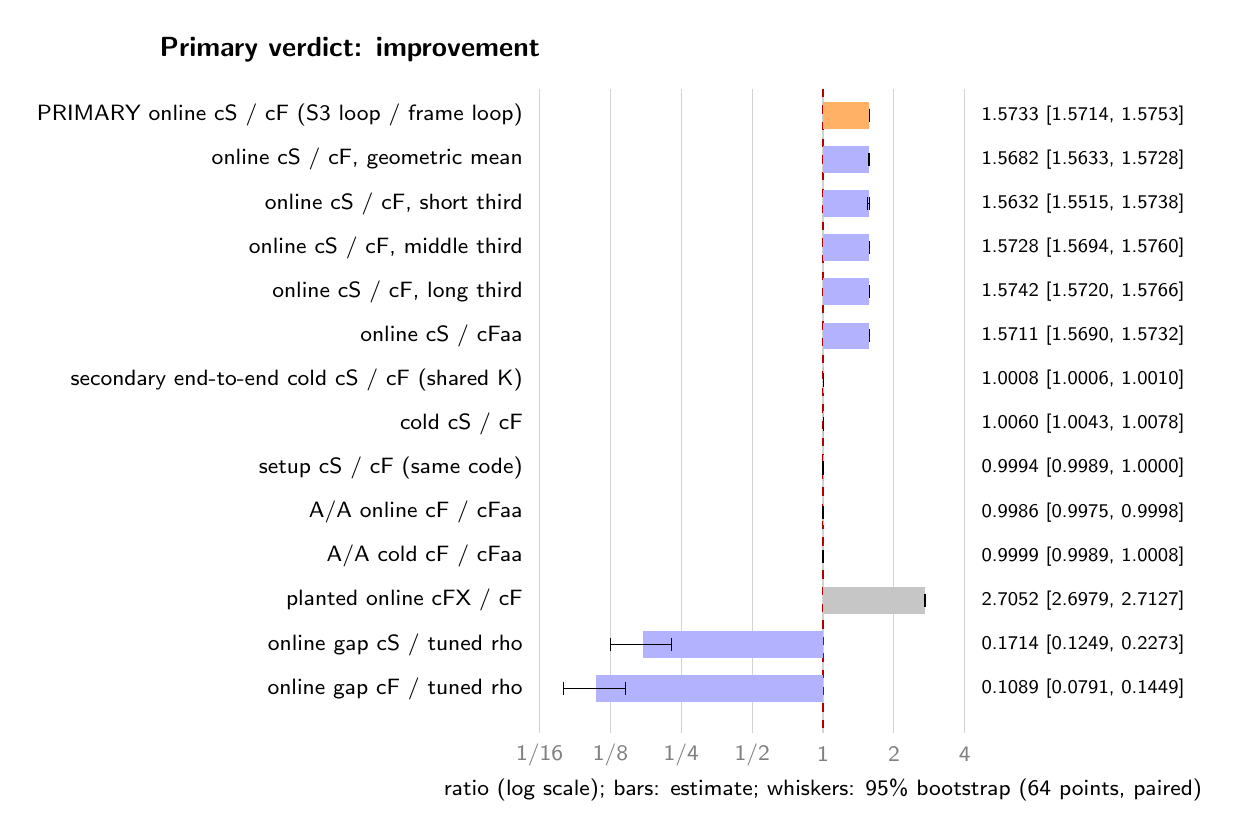
\begin{tikzpicture}[font=\sffamily\footnotesize,x=9mm,y=-5.6mm]
\draw[gray!35] (-4.0000,-0.6) -- (-4.0000,14); \node[gray] at (-4.0000,14.5) {1/16};
\draw[gray!35] (-3.0000,-0.6) -- (-3.0000,14); \node[gray] at (-3.0000,14.5) {1/8};
\draw[gray!35] (-2.0000,-0.6) -- (-2.0000,14); \node[gray] at (-2.0000,14.5) {1/4};
\draw[gray!35] (-1.0000,-0.6) -- (-1.0000,14); \node[gray] at (-1.0000,14.5) {1/2};
\draw[gray!35] (0.0000,-0.6) -- (0.0000,14); \node[gray] at (0.0000,14.5) {1};
\draw[gray!35] (1.0000,-0.6) -- (1.0000,14); \node[gray] at (1.0000,14.5) {2};
\draw[gray!35] (2.0000,-0.6) -- (2.0000,14); \node[gray] at (2.0000,14.5) {4};
\draw[red!70!black,dashed] (0,-0.6) -- (0,14);
\node at (0,15.3) {ratio (log scale); bars: estimate; whiskers: 95\% bootstrap (64 points, paired)};
\node[anchor=west,font=\sffamily\bfseries] at (-9.5,-1.5) {Primary verdict: improvement};
\node[anchor=east] at (-4.1000,0) {PRIMARY online cS / cF (S3 loop / frame loop)};
\fill[orange!60] (0,-0.300000) rectangle (0.6538,0.300000);
\draw (0.6520,0) -- (0.6557,0); \draw (0.6520,-0.150000) -- (0.6520,0.150000); \draw (0.6557,-0.150000) -- (0.6557,0.150000);
\node[anchor=west,font=\sffamily\scriptsize] at (2.1000,0) {1.5733 [1.5714, 1.5753]};
\node[anchor=east] at (-4.1000,1) {online cS / cF, geometric mean};
\fill[blue!30] (0,0.700000) rectangle (0.6491,1.300000);
\draw (0.6446,1) -- (0.6533,1); \draw (0.6446,0.850000) -- (0.6446,1.150000); \draw (0.6533,0.850000) -- (0.6533,1.150000);
\node[anchor=west,font=\sffamily\scriptsize] at (2.1000,1) {1.5682 [1.5633, 1.5728]};
\node[anchor=east] at (-4.1000,2) {online cS / cF, short third};
\fill[blue!30] (0,1.700000) rectangle (0.6445,2.300000);
\draw (0.6336,2) -- (0.6542,2); \draw (0.6336,1.850000) -- (0.6336,2.150000); \draw (0.6542,1.850000) -- (0.6542,2.150000);
\node[anchor=west,font=\sffamily\scriptsize] at (2.1000,2) {1.5632 [1.5515, 1.5738]};
\node[anchor=east] at (-4.1000,3) {online cS / cF, middle third};
\fill[blue!30] (0,2.700000) rectangle (0.6533,3.300000);
\draw (0.6502,3) -- (0.6563,3); \draw (0.6502,2.850000) -- (0.6502,3.150000); \draw (0.6563,2.850000) -- (0.6563,3.150000);
\node[anchor=west,font=\sffamily\scriptsize] at (2.1000,3) {1.5728 [1.5694, 1.5760]};
\node[anchor=east] at (-4.1000,4) {online cS / cF, long third};
\fill[blue!30] (0,3.700000) rectangle (0.6546,4.300000);
\draw (0.6526,4) -- (0.6568,4); \draw (0.6526,3.850000) -- (0.6526,4.150000); \draw (0.6568,3.850000) -- (0.6568,4.150000);
\node[anchor=west,font=\sffamily\scriptsize] at (2.1000,4) {1.5742 [1.5720, 1.5766]};
\node[anchor=east] at (-4.1000,5) {online cS / cFaa};
\fill[blue!30] (0,4.700000) rectangle (0.6518,5.300000);
\draw (0.6499,5) -- (0.6537,5); \draw (0.6499,4.850000) -- (0.6499,5.150000); \draw (0.6537,4.850000) -- (0.6537,5.150000);
\node[anchor=west,font=\sffamily\scriptsize] at (2.1000,5) {1.5711 [1.5690, 1.5732]};
\node[anchor=east] at (-4.1000,6) {secondary end-to-end cold cS / cF (shared K)};
\fill[blue!30] (0,5.700000) rectangle (0.0011,6.300000);
\draw (0.0008,6) -- (0.0015,6); \draw (0.0008,5.850000) -- (0.0008,6.150000); \draw (0.0015,5.850000) -- (0.0015,6.150000);
\node[anchor=west,font=\sffamily\scriptsize] at (2.1000,6) {1.0008 [1.0006, 1.0010]};
\node[anchor=east] at (-4.1000,7) {cold cS / cF};
\fill[blue!30] (0,6.700000) rectangle (0.0086,7.300000);
\draw (0.0062,7) -- (0.0113,7); \draw (0.0062,6.850000) -- (0.0062,7.150000); \draw (0.0113,6.850000) -- (0.0113,7.150000);
\node[anchor=west,font=\sffamily\scriptsize] at (2.1000,7) {1.0060 [1.0043, 1.0078]};
\node[anchor=east] at (-4.1000,8) {setup cS / cF (same code)};
\fill[blue!30] (0,7.700000) rectangle (-0.0008,8.300000);
\draw (-0.0016,8) -- (0.0000,8); \draw (-0.0016,7.850000) -- (-0.0016,8.150000); \draw (0.0000,7.850000) -- (0.0000,8.150000);
\node[anchor=west,font=\sffamily\scriptsize] at (2.1000,8) {0.9994 [0.9989, 1.0000]};
\node[anchor=east] at (-4.1000,9) {A/A online cF / cFaa};
\fill[gray!45] (0,8.700000) rectangle (-0.0020,9.300000);
\draw (-0.0037,9) -- (-0.0003,9); \draw (-0.0037,8.850000) -- (-0.0037,9.150000); \draw (-0.0003,8.850000) -- (-0.0003,9.150000);
\node[anchor=west,font=\sffamily\scriptsize] at (2.1000,9) {0.9986 [0.9975, 0.9998]};
\node[anchor=east] at (-4.1000,10) {A/A cold cF / cFaa};
\fill[gray!45] (0,9.700000) rectangle (-0.0001,10.300000);
\draw (-0.0015,10) -- (0.0011,10); \draw (-0.0015,9.850000) -- (-0.0015,10.150000); \draw (0.0011,9.850000) -- (0.0011,10.150000);
\node[anchor=west,font=\sffamily\scriptsize] at (2.1000,10) {0.9999 [0.9989, 1.0008]};
\node[anchor=east] at (-4.1000,11) {planted online cFX / cF};
\fill[gray!45] (0,10.700000) rectangle (1.4358,11.300000);
\draw (1.4318,11) -- (1.4397,11); \draw (1.4318,10.850000) -- (1.4318,11.150000); \draw (1.4397,10.850000) -- (1.4397,11.150000);
\node[anchor=west,font=\sffamily\scriptsize] at (2.1000,11) {2.7052 [2.6979, 2.7127]};
\node[anchor=east] at (-4.1000,12) {online gap cS / tuned rho};
\fill[blue!30] (0,11.700000) rectangle (-2.5446,12.300000);
\draw (-3.0014,12) -- (-2.1374,12); \draw (-3.0014,11.850000) -- (-3.0014,12.150000); \draw (-2.1374,11.850000) -- (-2.1374,12.150000);
\node[anchor=west,font=\sffamily\scriptsize] at (2.1000,12) {0.1714 [0.1249, 0.2273]};
\node[anchor=east] at (-4.1000,13) {online gap cF / tuned rho};
\fill[blue!30] (0,12.700000) rectangle (-3.1984,13.300000);
\draw (-3.6601,13) -- (-2.7865,13); \draw (-3.6601,12.850000) -- (-3.6601,13.150000); \draw (-2.7865,12.850000) -- (-2.7865,13.150000);
\node[anchor=west,font=\sffamily\scriptsize] at (2.1000,13) {0.1089 [0.0791, 0.1449]};
\end{tikzpicture}
\end{document}
